
    \begin{center}
    \end{center}
\end{figure}

        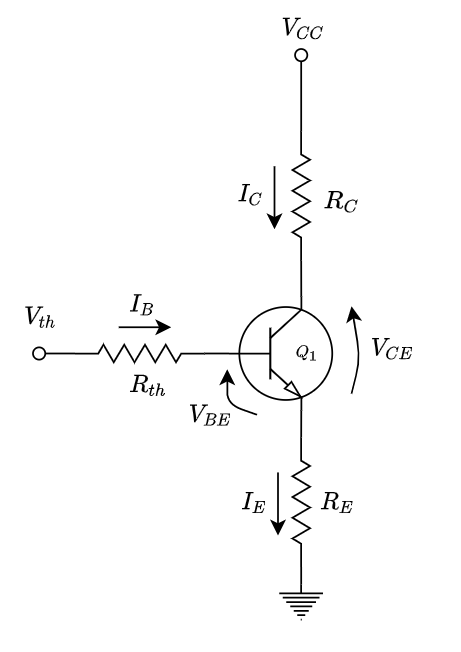
\includegraphics[width=0.3\textwidth]{polarizacion_de_base/Imagenes/circuito_polarizacion_base_thevenin.png}


En el caso 1, la tensión de entrada sería suficiente para polarizar el Diodo zener a su 

\section{Selección de componentes}

Contando entonces con el transistor bipolar BC547, se buscan los valores para $R_c$, $R_b$ y $R_e$ tal que se cumplan las condiciones de diseño.
En este caso se desea $I_c =  2mA$. Es necesario buscar en la hoja de datos del transistor los datos de la tabla INSERTAR REFERENCIA A TABLA.
\begin{table}[]
    \begin{tabular}{l|l|l|l}
                  & Min  & Típica & Máximo \\ \hline
    $\beta$       & 100  &        & 800    \\ \hline
    $V_{BEon}$    & 0.58 & 0.66   & 0.7    \\ \hline
    $V_{CEsat}$   &      & 0.09   & 0.25  
    \end{tabular} \label{table:parametros transistor}
